\documentclass[12pt,a4paper]{article}

\usepackage[top=1.5cm, bottom=1.8cm, left=1.2cm, right=1.2cm, landscape]{geometry}
\usepackage{tikz}
\usepackage{xcolor}
\usepackage[T1]{fontenc}
\usepackage{caption}
\usepackage{float}

\usetikzlibrary{arrows.meta, fit, backgrounds, calc}

\definecolor{TealFill}    {HTML}{E1F5EE}
\definecolor{TealStroke}  {HTML}{0F6E56}
\definecolor{PurpleFill}  {HTML}{EEEDFE}
\definecolor{PurpleStroke}{HTML}{534AB7}
\definecolor{BlueFill}    {HTML}{E6F1FB}
\definecolor{BlueStroke}  {HTML}{185FA5}
\definecolor{AmberFill}   {HTML}{FAEEDA}
\definecolor{AmberStroke} {HTML}{854F0B}
\definecolor{GreenFill}   {HTML}{EAF3DE}
\definecolor{GreenStroke} {HTML}{3B6D11}
\definecolor{SigGray}     {HTML}{5F5E5A}
\definecolor{BypassRed}   {HTML}{993C1D}

\tikzset{
  block/.style={
    draw, rounded corners=4pt,
    minimum width=4.4cm, minimum height=1.3cm,
    align=center, line width=0.5pt, inner sep=6pt,
    font=\small\bfseries,
  },
  stagebox/.style={
    draw, rounded corners=8pt, line width=0.6pt, dashed, inner sep=14pt,
  },
  notebox/.style={
    draw=BypassRed, rounded corners=4pt, line width=0.5pt,
    fill=white, inner sep=7pt, align=left,
    font=\fontsize{7}{9}\selectfont, text=BypassRed,
  },
  ioblock/.style ={block, fill=TealFill,   draw=TealStroke,   text=TealStroke},
  s1block/.style ={block, fill=PurpleFill, draw=PurpleStroke, text=PurpleStroke},
  s2block/.style ={block, fill=BlueFill,   draw=BlueStroke,   text=BlueStroke},
  cfgblock/.style={block, fill=AmberFill,  draw=AmberStroke,  text=AmberStroke,
                   minimum width=3.2cm, minimum height=1.0cm},
  outblock/.style={block, fill=GreenFill,  draw=GreenStroke,  text=GreenStroke,
                   minimum width=3.0cm},
  sig/.style={
    -{Stealth[length=5pt,width=4pt]}, color=SigGray, line width=0.6pt,
  },
  sigdash/.style={
    -{Stealth[length=4pt,width=3.5pt]}, color=SigGray, line width=0.5pt, dashed,
  },
  lbl/.style={
    font=\fontsize{6.5}{8}\selectfont\itshape,
    text=SigGray, fill=white, inner sep=1.5pt,
  },
}

\newcommand{\sub}[1]{\\[2pt]{\fontsize{6.5}{8}\selectfont\mdseries\color{SigGray}#1}}

\begin{document}
\pagestyle{empty}

\begin{figure}[H]
\centering
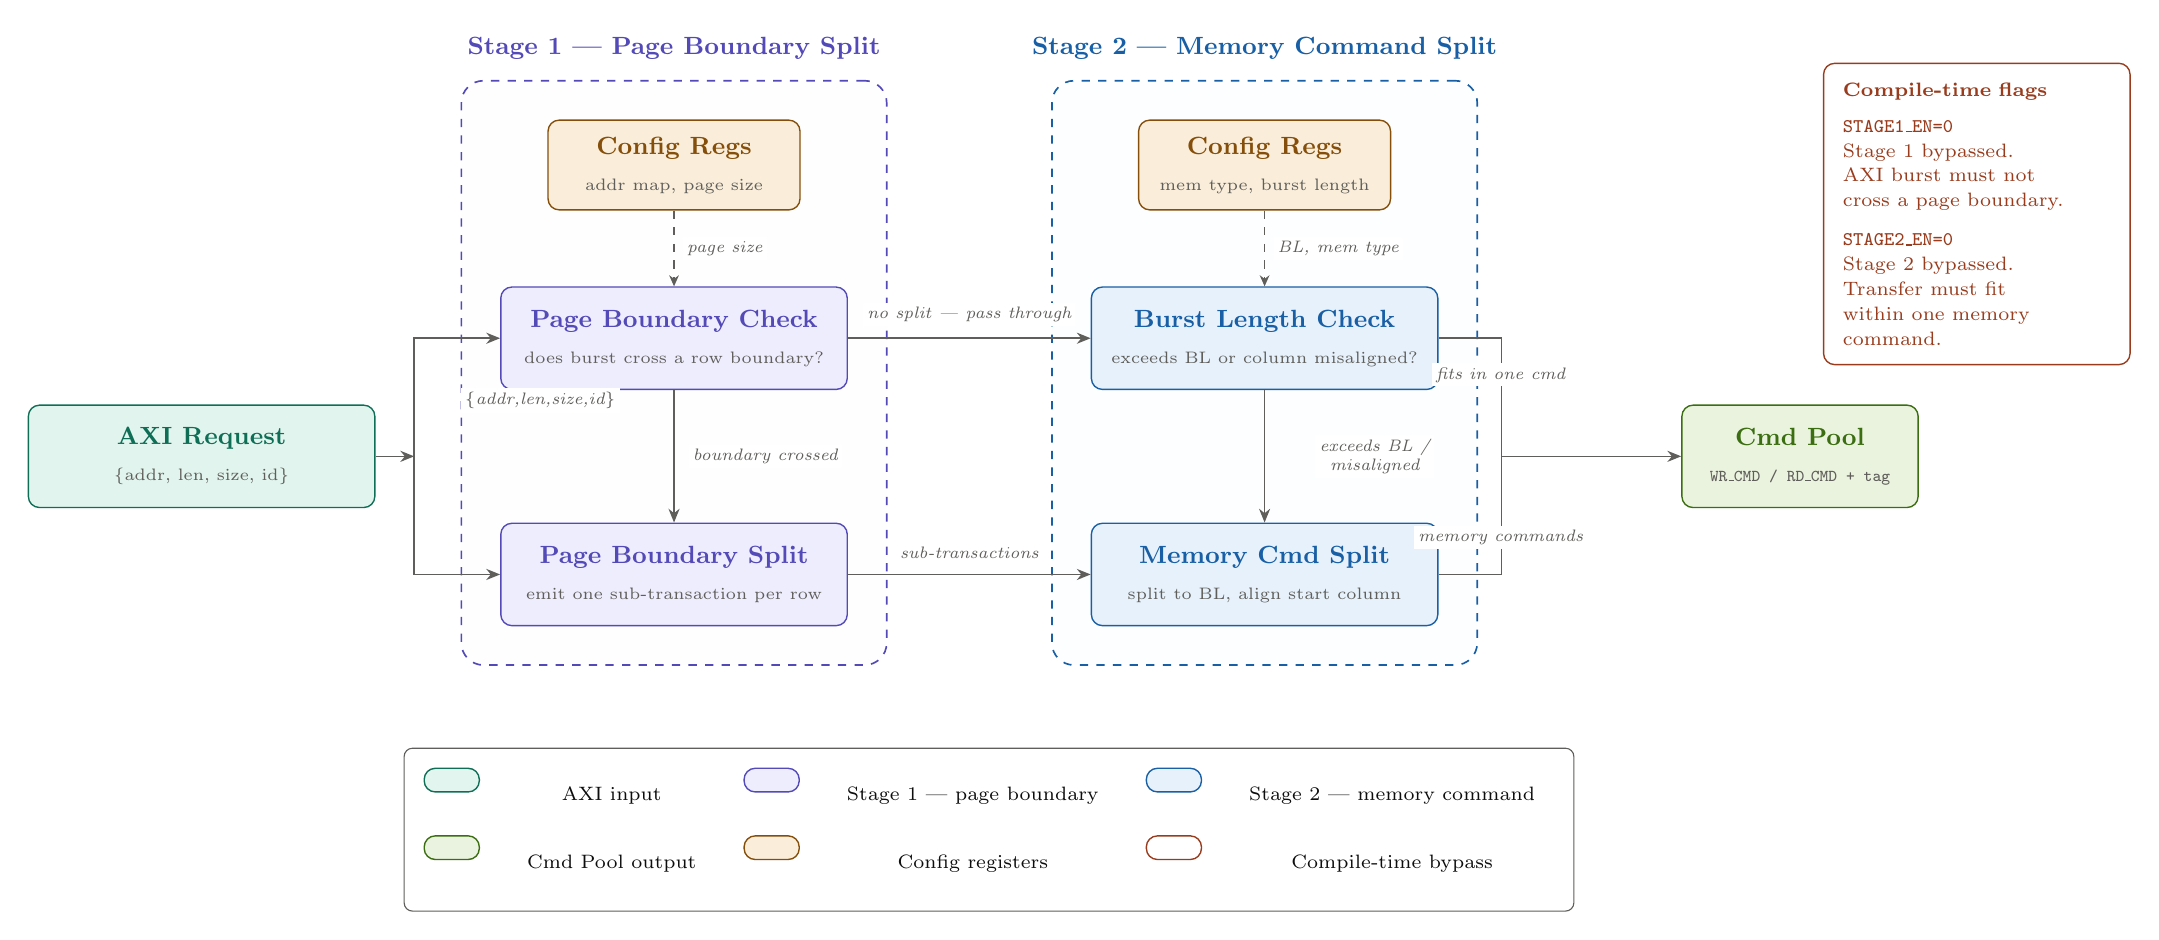
\begin{tikzpicture}

% ── Nodes ─────────────────────────────────────────────────────────────────
% Wide layout: S1 at x=7.5, S2 at x=15.0, OUT at x=21.5, NOTE at x=23.0
\node[ioblock]  (IN)   at ( 1.5, -1.5) {AXI Request\sub{\{addr, len, size, id\}}};
\node[cfgblock] (CFG1) at ( 7.5,  2.2) {Config Regs\sub{addr map, page size}};
\node[s1block]  (S1C)  at ( 7.5,  0.0) {Page Boundary Check\sub{does burst cross a row boundary?}};
\node[s1block]  (S1S)  at ( 7.5, -3.0) {Page Boundary Split\sub{emit one sub-transaction per row}};
\node[cfgblock] (CFG2) at (15.0,  2.2) {Config Regs\sub{mem type, burst length}};
\node[s2block]  (S2C)  at (15.0,  0.0) {Burst Length Check\sub{exceeds BL or column misaligned?}};
\node[s2block]  (S2S)  at (15.0, -3.0) {Memory Cmd Split\sub{split to BL, align start column}};
% Cmd Pool pushed right so labels between S2 and OUT have room
\node[outblock] (OUT)  at (21.8, -1.5) {Cmd Pool\sub{\texttt{WR\_CMD / RD\_CMD + tag}}};

% ── Signals ───────────────────────────────────────────────────────────────

% IN -> fork -> S1C / S1S
% Fork at x=4.2; label goes BELOW the horizontal segment into S1C
\coordinate (FORK) at (4.2, -1.5);
\draw[sig] (IN.east) -- (FORK);
\draw[sig] (FORK) |- (S1C.west);
\draw[sig] (FORK) |- (S1S.west);
% Label below the arm going to S1C, anchored at midpoint of arm
\node[lbl, anchor=north] at (5.8, -0.62) {\{addr,len,size,id\}};

% S1C -> S1S
\draw[sig] (S1C.south) -- (S1S.north)
  node[lbl, midway, right=5pt] {boundary crossed};

% S1C -> S2C  top rail
\draw[sig] (S1C.east) -- (S2C.west)
  node[lbl, midway, above=4pt] {no split --- pass through};

% S1S -> S2S  bottom rail
\draw[sig] (S1S.east) -- (S2S.west)
  node[lbl, midway, above=4pt] {sub-transactions};

% S2C -> S2S
\draw[sig] (S2C.south) -- (S2S.north);
\node[lbl, align=center, anchor=center] at (16.4, -1.5) {exceeds BL /\\[-1pt]misaligned};

% S2C and S2S merge into OUT.west — mirror of IN fork on the left
% Merge point at x=19.5 (midway between S2 right edge ~17.2 and OUT left ~20.3)
\coordinate (MERGE2) at (19.5, -1.5);
\draw[SigGray, line width=0.6pt] (S2C.east) -- ++(0.8,0) |- (MERGE2);
\draw[SigGray, line width=0.6pt] (S2S.east) -- ++(0.8,0) |- (MERGE2);
\draw[sig] (MERGE2) -- (OUT.west);
\node[lbl, anchor=south] at (18.0, -0.62) {fits in one cmd};
\node[lbl, anchor=north] at (18.0, -2.38) {memory commands};

% Config regs
\draw[sigdash] (CFG1.south) -- (S1C.north)
  node[lbl, midway, right=3pt] {page size};
\draw[sigdash] (CFG2.south) -- (S2C.north)
  node[lbl, midway, right=3pt] {BL, mem type};

% ── Stage containers ──────────────────────────────────────────────────────
\begin{scope}[on background layer]
  \node[
    stagebox, fill=PurpleFill, fill opacity=0.07, draw=PurpleStroke,
    fit=(CFG1)(S1C)(S1S),
    label={[font=\small\bfseries, text=PurpleStroke, yshift=4pt]
           above:Stage 1 \textemdash\ Page Boundary Split},
  ] (BOX1) {};
  \node[
    stagebox, fill=BlueFill, fill opacity=0.07, draw=BlueStroke,
    fit=(CFG2)(S2C)(S2S),
    label={[font=\small\bfseries, text=BlueStroke, yshift=4pt]
           above:Stage 2 \textemdash\ Memory Command Split},
  ] (BOX2) {};
\end{scope}

% ── Note box: placed below and right of OUT, no overlap ───────────────────
\node[notebox, text width=3.4cm, anchor=north east] at (26.0, 3.5) {%
  \textbf{Compile-time flags}\\[4pt]
  \texttt{STAGE1\_EN=0}\\
  Stage~1 bypassed.\\
  AXI burst must not\\
  cross a page boundary.\\[5pt]
  \texttt{STAGE2\_EN=0}\\
  Stage~2 bypassed.\\
  Transfer must fit\\
  within one memory\\
  command.%
};

% ── Legend ────────────────────────────────────────────────────────────────
\matrix (LEG) [
  draw=SigGray, rounded corners=3pt, line width=0.4pt,
  fill=white, fill opacity=0.95,
  inner sep=7pt, column sep=10pt, row sep=4pt,
  every node/.style={font=\fontsize{7.5}{9}\selectfont},
  at={(11.5,-5.2)}, anchor=north,
] {
  \node[ioblock,  minimum width=0.7cm, minimum height=0.3cm, inner sep=2pt]{}; &
  \node{AXI input}; &
  \node[s1block,  minimum width=0.7cm, minimum height=0.3cm, inner sep=2pt]{}; &
  \node{Stage 1 — page boundary}; &
  \node[s2block,  minimum width=0.7cm, minimum height=0.3cm, inner sep=2pt]{}; &
  \node{Stage 2 — memory command}; \\
  \node[outblock, minimum width=0.7cm, minimum height=0.3cm, inner sep=2pt]{}; &
  \node{Cmd Pool output}; &
  \node[cfgblock, minimum width=0.7cm, minimum height=0.3cm, inner sep=2pt]{}; &
  \node{Config registers}; &
  \node[notebox,  minimum width=0.7cm, minimum height=0.3cm, inner sep=2pt]{}; &
  \node{Compile-time bypass}; \\
};

\end{tikzpicture}

\caption{%
  \textbf{Burst Splitter} internal pipeline.
  Stage~1 splits an AXI Request at row (page) boundaries into
  linear transactions each confined to a single row.
  Stage~2 divides each into memory commands sized to the configured
  burst length and aligned to the start column address.
  Both stages are individually enabled or disabled at compile time.
}
\label{fig:burst-splitter}
\end{figure}
\end{document}
